% Created 2016-08-11 Thu 13:30
\documentclass[twoside]{article}
\usepackage[utf8]{inputenc}
\usepackage[T1]{fontenc}
\usepackage{fixltx2e}
\usepackage{graphicx}
\usepackage{grffile}
\usepackage{longtable}
\usepackage{wrapfig}
\usepackage{rotating}
\usepackage[normalem]{ulem}
\usepackage{amsmath}
\usepackage{textcomp}
\usepackage{amssymb}
\usepackage{capt-of}
\usepackage{hyperref}
\usepackage{setspace}
\doublespacing
\usepackage{titletoc}
\usepackage{mathtools}
\usepackage[innermargin=1.5in,outermargin=1.25in,vmargin=1.25in]{geometry}
\usepackage[authordate,bibencoding=utf8,strict,backend=biber,doi=false,isbn=false,url=false]{biblatex-chicago}
\hypersetup{colorlinks=true,citecolor=black,linkcolor=black,citebordercolor={0 1 0},linktocpage,pdfstartview=FitH,anchorcolor=black,filecolor=black,menucolor=black,urlcolor=black}
\addbibresource{/home/japhir/minimal_tex/minimal.bib}
\newcommand{\dtC}{\ce{\delta^{13}C}}
\newcommand{\deO}{\ce{\delta^{18}O}}
\setcounter{secnumdepth}{2}
\author{It's me\thanks{my@email.me}}
\date{August 2016}
\title{Cat Title}
\hypersetup{
 pdfauthor={It's me},
 pdftitle={Cat Title},
 pdfkeywords={},
 pdfsubject={},
 pdfcreator={Emacs 24.5.1 (Org mode 8.3.5)}, 
 pdflang={English}}
\begin{document}

\maketitle
\begin{abstract}
This is the abstract.
\end{abstract}

\setcounter{tocdepth}{2}
\tableofcontents

\section{Introduction}
\label{sec:orgheadline1}

See Figure \ref{fig:orgparagraph1}
\section{Material and Methods}
\label{sec:orgheadline2}

This has a reference using \texttt{cite} \cite{Cats2016}. Also a \texttt{textcite} \textcite{Cats2016} and a \texttt{parencite} \parencite{Cats2016}.
\begin{figure}[htbp]
\centering
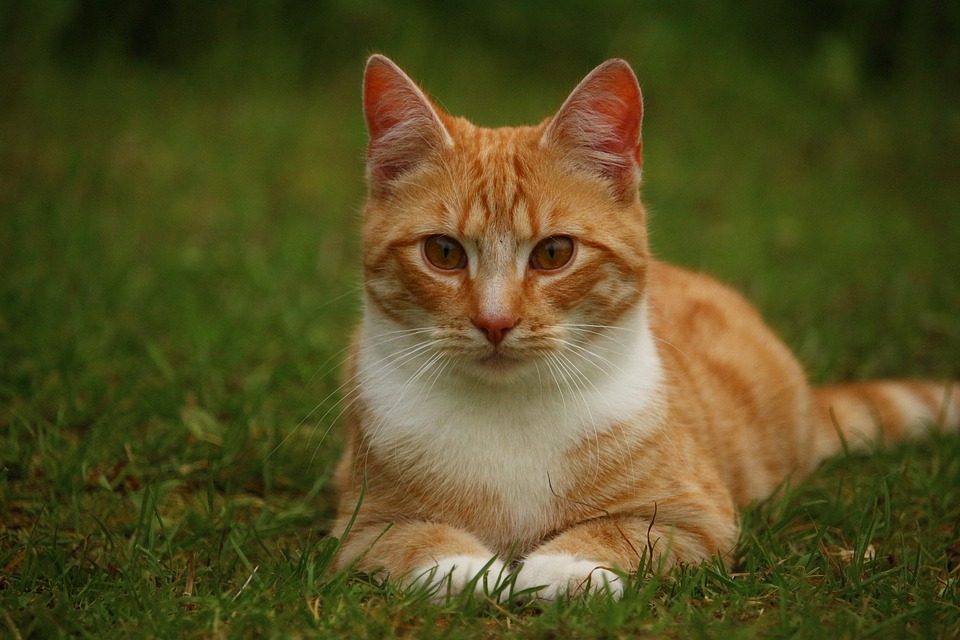
\includegraphics[width=\textwidth]{cats.jpg}
\caption{\label{fig:orgparagraph1}
Cat!}
\end{figure}

\section{Results}
\label{sec:orgheadline3}

\section{Discussion}
\label{sec:orgheadline4}

\section{Acknowledgements}
\label{sec:orgheadline5}

\section{References}
\label{sec:orgheadline6}

\printbibliography
\end{document}